
\section{Plugin} %interoperability?

In order to improve the deployment and usage of the refactoring tool a plugin
for DrRacket was created.
DrRacket has several advantages and the plugin support is another one, because
it allows a simple integration with DrRacket itself a simple managing interface.
Another advantage is the incorporation with git. A plugin can be a link for a git
repository and because of that it becomes simple to keep the refactoring tool up to date.

However, the main reason to create a plugin is to become independent from DrRacket
internal changes.

%TODO TODO intro? TODO TODO TODO
Refactoring static languages
As we do not explore type information to do refactoring operations to static typified
programing languages we can not say that we do refactoring for static langauges.
However, there are fragments/subsets of those languages that may be refactored by our
framework. Those fragments are parts of the code that can be reason upon without using
the type information, for example:
%That subset can be refactored. %TODO explain further!
\section{FrameWork}
Since refactoring tools often require the same information about the program, such as
the AST and the def-use-relations, and therefore they have similar architecture.
This similarity between refactoring tools creates the possibility of reusing some modules
instead of creating every module from scratch therefore making refactoring tools
development become a lot faster.
Having a framework to create refactoring tools can ease up the pain and in addition
it is posssible to share features created for a refactoring tool with the other refactoring
tools developed using the framework, for example: .
Since we desire to create a refactoring tool targeted to beginner programmers with
specialized refactoring operations and we want such refactoring tool to be available
for several languages used in introductory courses around the world and not just for
Racket programming language.
Creating a framework for refactoring tools increases both the speed and the simplicity (??)
of creating a refactoring tool and therefore it is able to provide the features already available
for one refactoring tool in the others without extra effort. Such features highly improve
the usefulness of the refactoring tool, for example the highlight of possible refactoring
operations, the previewing of the result and support to detect duplicated code.


 %[TODO Explain META-LANGUAGE]
 Impementing the framework in Racket combined with the implmented languages for DrRacket is what does the trick,
 since we use the implemetnation as a meta-language which creates syntax objects as the ones used to represent the racket language.
  Being the meta-language a language that are
 composed only by syntax elements is a huge advantage to compute effortless new
 refactoring operations for new languages when compared with the necessary effort to create
 the refactoring operations directly for that language.

Ideally we should only have refactoring operations for the meta-language which represents
all languages. And then specialized pretty printers to output the changes in the
desireble language.
However, since we instead of having a general representation that can represent all the languages
supported we have the languages represented in Racket's syntax objects we can not do that.

We indeed have a meta-language that abstracts all the supported languages and
we have trully language independent refactoring operations. However, it is only
for a small set of refactoring opeartions, the more simple ones. We did it like
this because we would lose some of the possible refactoring operations or we would
have to have a lot of concerns. And since we have a restrict amount of time, having
a meta-language that have language-independent refactoring operations combined
with the "semi-meta-languages" that have similar refactoring operations but
language dependent and therefore more specialized.

With this we do not have a language-independent framework. However we have a framework
for refactoring operations, even tough that is more aimed at dynamic and functional languages.
Framework architecture.%FIXME this is super weird
\begin{figure}[h]
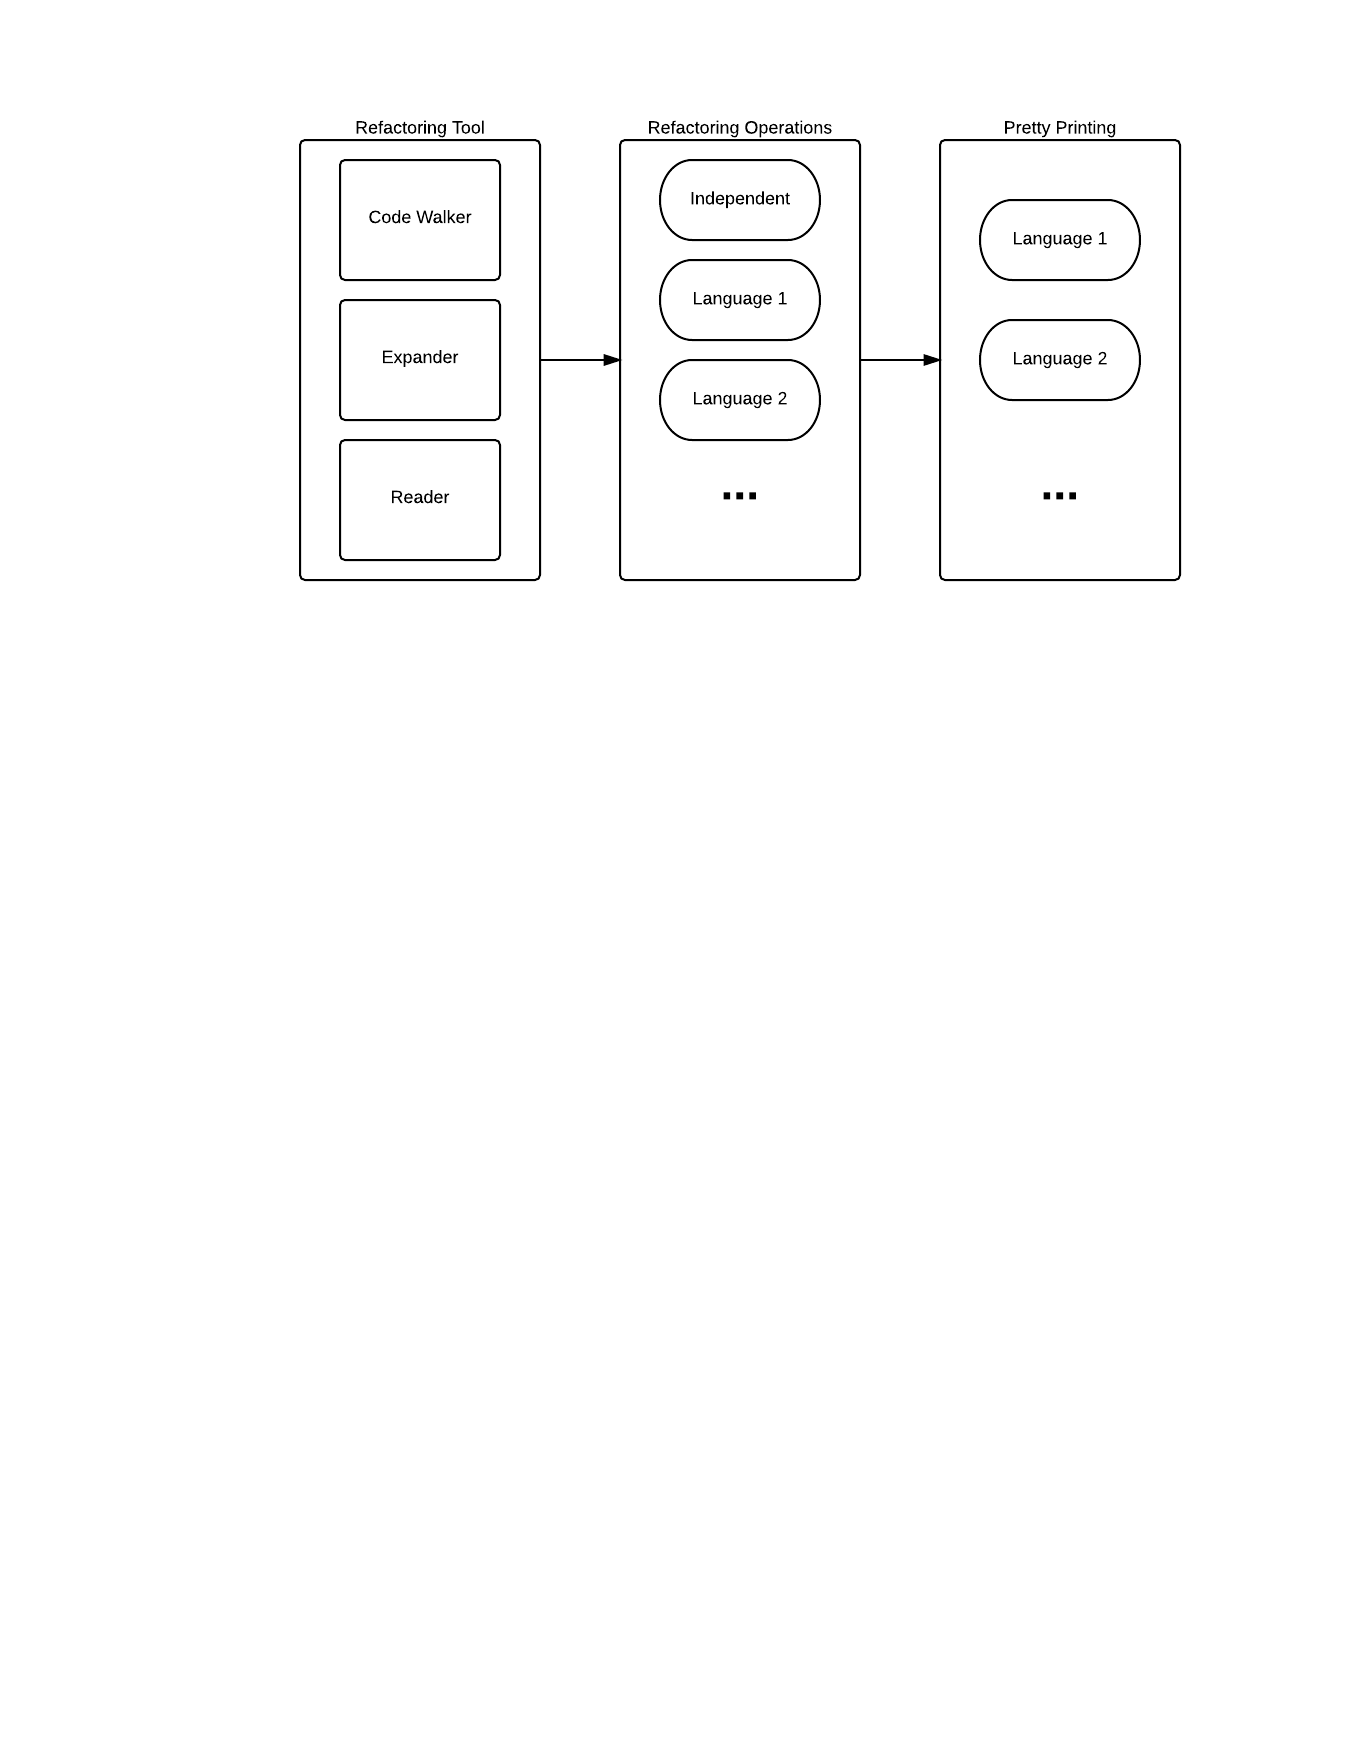
\includegraphics[width=8cm]{../framework-arch2.png}
\label{fig:framework}
\end{figure}

As it is described in Figure~\ref{fig:framework} we have a module that provides
independent refactoring operations and a module for each language supported that
have specialized refactoring operations. We also have pretty-printing modules for
each supported language.

We already have refactoring operations for Racket, Python, and Processing. We choose
this languages because they are already implemented in Racket and they are both
often used by beginners.


\subsection{Statement based languages}
This Framework was build with a base of expression based languages. The flow of
the program is needed to decide whether or not a refactoring can be correctly done
or even to decide where and how many returns a function needs. However this could
be minimized with a PDG (program depedence graph) that has the control flow information
needed to compute correct refactorings.

\subsection{Language Independent refactoring operations}
Creating a fully language independent refactoring tool is difficult since programming
languages differ semantically from each other, even some operations that are semantically
equal for most of the cases, for the cases that they are not semantically equal makes it very
difficult to do a general refactoring operation.
%TODO give an example. (+ in python?) (< ?)
However, for simple refactoring opeartions, which do not require much program semantics,
it is possible to have language independente refactoring operations in a meta-language that
represents the semanatic of the other implemented languages. %TODO CHECK THIS

\subsection{Language dependent refactoring operations}
It is necessary to have refactoring operations that are language dependent, since
some refactoring operatons have particular cases for each supported language.
Having specific refactoring operations, language dependent ones, it is possible
to implement some useful refactoring operations in a simple way that otherwise would
be too complex.
%TODO give an example

\section{Features} %talk about one feature fits all
how easy it is to add new refactoring operations and languages
The framework it is simply to use, it is only necessary to have a specification file
of each refactoring operation.
That file must have a function that receives two arguments,
one is the AST of the program and the other is the def-use-relation.
This information makes it possible to have several refactoring operations that help
the programmer.
what was "reused"
everything except the refactoring operations itself.
the advantages of that
This Framework makes it easier to implement refactoring operations for dynamic languages,
with only the catch that they have to be implemented for DrRacket. Helping minimizing
the problem of the difficulty and lacking of refactoring operations for dynamic languages.
(for at least every language implemented for DrRacket)

Automatic detection
Preview
duplicated code detection
\section{Tool Maintenance} %Framework maintenance!
%Developer Point of view
%%%% Nor for the paper tough %%%%
%%automatic might help save work when the user nows what exactly the tool will do.

%This feature combined with the automatic suggesting is a huge help to do the
%evaluation of this refactoring tool and to use in battery tests.


A refactoring tool is a quite complex piece of software and therefore requires maintenance.
Automatic testing is used in general by developers to ensure that the software
is bug free for those test cases.
By having a way to automatically perform all the refactoring operations found,
the developer of a refactoring tool can test and ensure if the changes made did not introduce
bugs in other refactoring operations of the refactoring tool.
One way to automatic test the refactoring operations is to apply every refactoring
operations possible to a piece of code. By having this possibility it is simpler
to the developer to create specific test cases that simplify tool maintenance.
In order to do this it is necessary to correctly identify all the possible refactoring
operations in one piece of code. Such operation is already implemented in the refactoring
tool, the automatic suggesting.
Therefore the remaining part of the algorithm is to apply all of those operations.
The trick part is  that every refactoring operation changes the AST, so after
applying one refactoring operation it is necessary to recompute the program AST.
By changing the AST the possible refactoring operations applicable also might change,
so it is necessary to recompute the AST.

%First the automated refactoring displays all the possible refactoring found thus making it easier
%to detect the refactoring operations in projects.
%It makes it easier to evaluate the need to do the refactoring and to evaluate
%if the refactoring tool (frameowork) is working correctly.
%Second the automatic refactoring makes it easier to test if the refactoring operations are correct (**** for a limited test cases ****)
%This is possible by running the test cases of the program before any refactoring.
%Then using automatic refactoring in the program that applies all the refactoring that the tool finds.
%And finally by running again the test cases of the program.
%After testing it with several (or huge) programs if every test passes (or the exact same tests, because refactoring operations should not fix bugs)
%we can consider that the refactoring operations are correct.

\section{Examples}  %evaluation?

\section{Analysis} %and conclusion
Combining the two approaches can simply create refactoring operations for several
languages targetted at beginner programmers. Some of this refactoring operations
are rather simple, when compared to more advanced ones, and some can even be reproduced
in a meta-language and therefore only implemented once for several programming languages.
For the rest of the refactoring operations they can be added to the dependent language
module in which it is possible to have the special cases covered.

With the combination usage of reader + expander + code-walker working for the several
implemented languages most of the work is already done and when combined with the
powerfulness offered by the syntax-parser it is possible to create refactoring operations
using only one line of code, e.g. %TODO add an example
Even having some refactoring operations that are more complex it is way quicker and
simpler only to have to implement the refactoring operation itself.
However, there is still lacking of program information that is rather useful for
statement based languages (or even object oriented ones?) which is program dependence.
%extract function for python + processing, atm is kinda tricky!
Having more program information available, such as the dependence, it is possible to
create even more complex refactoring operations which would be a great improvement.


%\section{Conclusion}

\section{Future Work}
Add a PDG to the framework.
Simplify adding langauges to the framework
Simplify create features for all languages.
Create an API??
